

\subsection{Field Orientated Control}
Multiple ways exist to control motors but in this project Field Orientated Control (FOC) has been chosen for its simplicity and ease of implementation. The idea behind FOC is to transform the three phase currents into a single vector in a rotating frame of reference that rotates with the same speed as the rotor. 
Perform the control in the rotating frame and then transform the controller signals back out into three phase signals which results in a control loop as can be seen on figure \ref{fig:Motor_model}.

\begin{figure} [H]
    \centering
    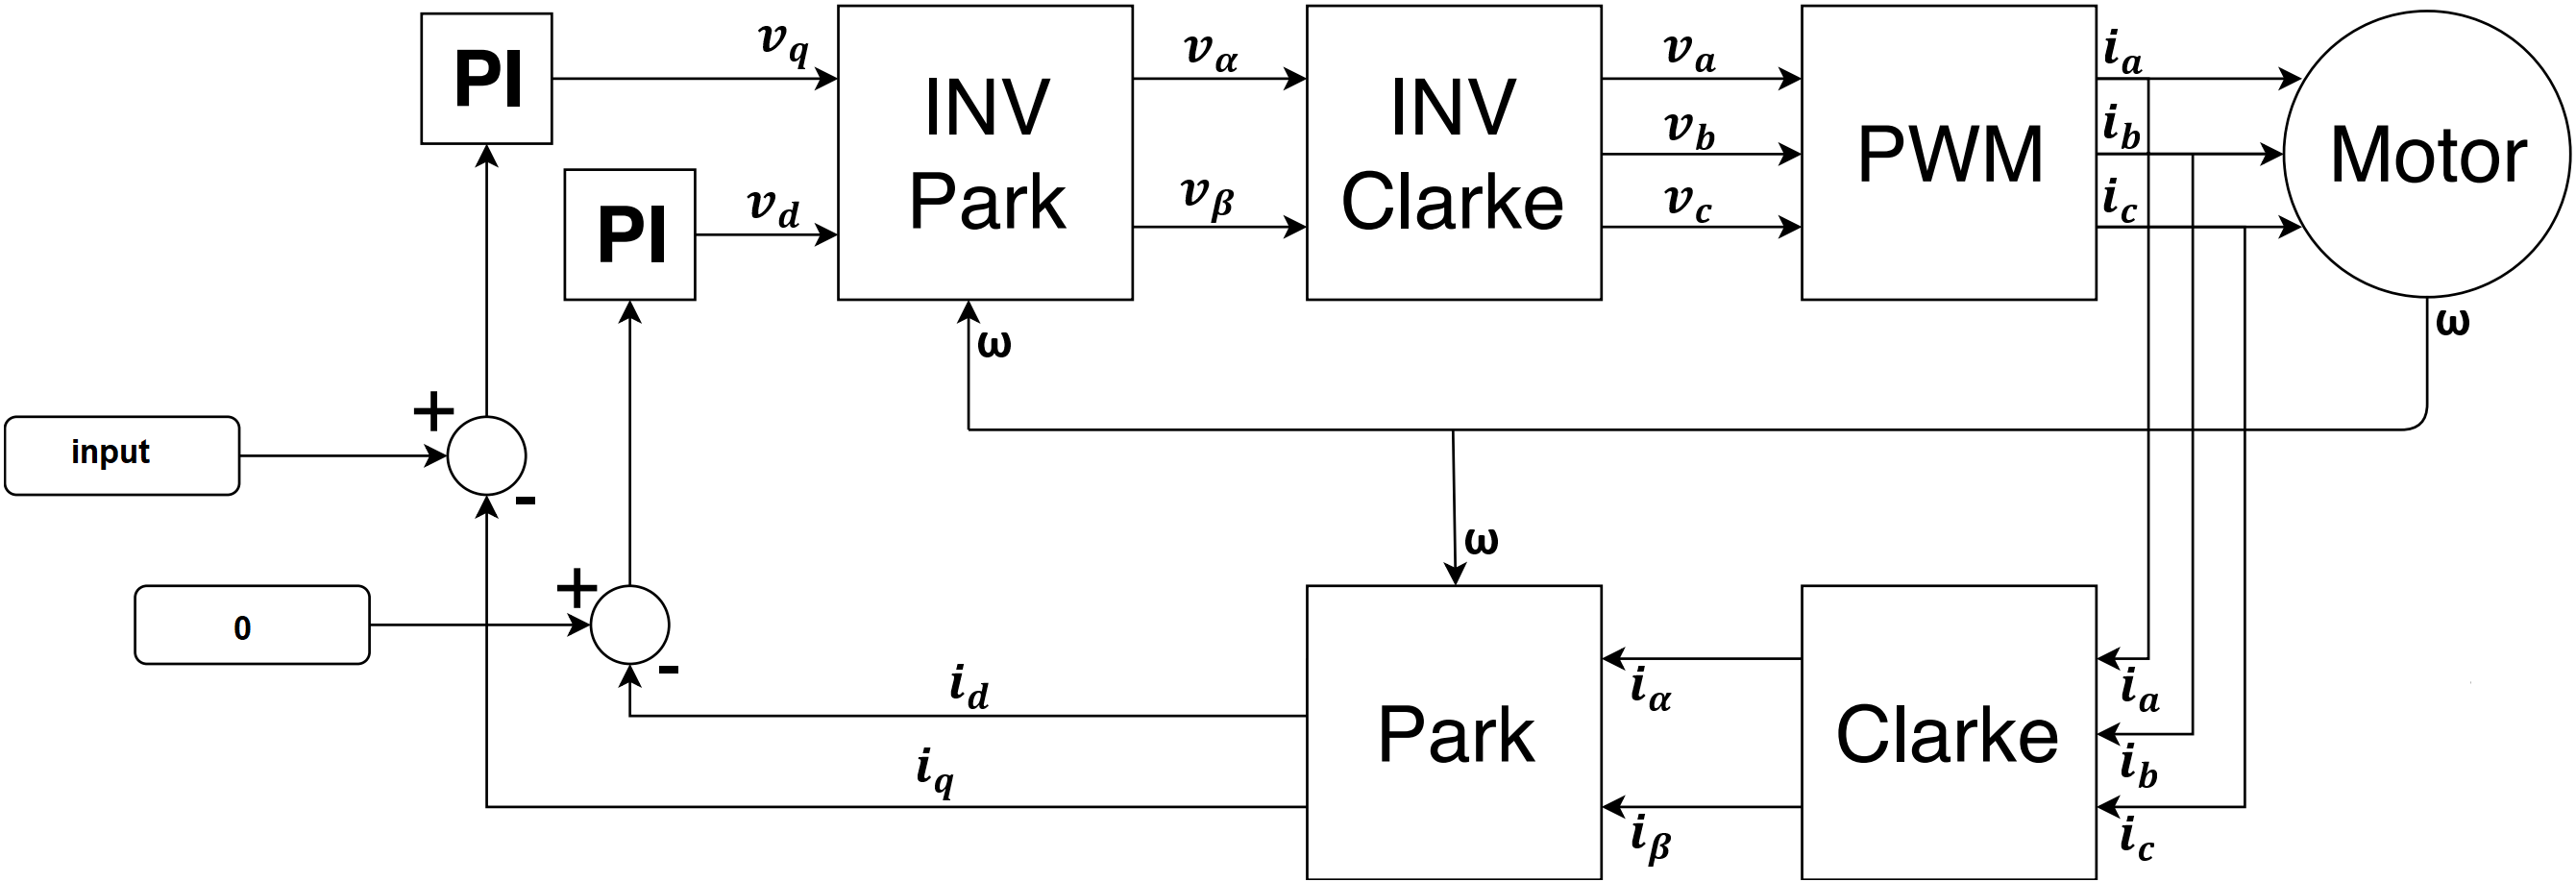
\includegraphics[scale=0.42]{pictures/control/udklip.PNG}
    \caption{Motor model used for the control as an overview.}
    \label{fig:Motor_model}
\end{figure} 

On the right the motor can be seen. The phase current out of the inverter is transformed into a rotating frame of reference by first performing a Clarke Transformation and then a Park Transformation. Out comes two signals $i_d$ and $i_q$ which goes into two individual controllers. FOC usually use PI controllers because only a proportional and a integrator part is needed. The motor torque is biggest when the electric field is perpendicular to the rotor position. The $i_d$ signal should always be $0$ because it resembles electric field not perpendicular to the rotor. Therefore it is subtracted with $0$ which makes $i_d$ the error and the signal is out into the PI controller. The $i_q$ resembles the electric field perpendicular to the rotor which is what produces the torque. Therefore this signal is compared with the input which is the target torque that comes from the torque pedal. After the PI controllers the two control signals in the rotating frame of reference are transformed back out into three phases with an Inverse Park Transformation and an Inverse Clarke Transformation. The signals can then be used to control the inverter.

